
%% bare_conf.tex
%% V1.4b
%% 2015/08/26
%% by Michael Shell
%% See:
%% http://www.michaelshell.org/
%% for current contact information.
%%
%% This is a skeleton file demonstrating the use of IEEEtran.cls
%% (requires IEEEtran.cls version 1.8b or later) with an IEEE
%% conference paper.
%%
%% Support sites:
%% http://www.michaelshell.org/tex/ieeetran/
%% http://www.ctan.org/pkg/ieeetran
%% and
%% http://www.ieee.org/

%%*************************************************************************
%% Legal Notice:
%% This code is offered as-is without any warranty either expressed or
%% implied; without even the implied warranty of MERCHANTABILITY or
%% FITNESS FOR A PARTICULAR PURPOSE! 
%% User assumes all risk.
%% In no event shall the IEEE or any contributor to this code be liable for
%% any damages or losses, including, but not limited to, incidental,
%% consequential, or any other damages, resulting from the use or misuse
%% of any information contained here.
%%
%% All comments are the opinions of their respective authors and are not
%% necessarily endorsed by the IEEE.
%%
%% This work is distributed under the LaTeX Project Public License (LPPL)
%% ( http://www.latex-project.org/ ) version 1.3, and may be freely used,
%% distributed and modified. A copy of the LPPL, version 1.3, is included
%% in the base LaTeX documentation of all distributions of LaTeX released
%% 2003/12/01 or later.
%% Retain all contribution notices and credits.
%% ** Modified files should be clearly indicated as such, including  **
%% ** renaming them and changing author support contact information. **
%%*************************************************************************


% *** Authors should verify (and, if needed, correct) their LaTeX system  ***
% *** with the testflow diagnostic prior to trusting their LaTeX platform ***
% *** with production work. The IEEE's font choices and paper sizes can   ***
% *** trigger bugs that do not appear when using other class files.       ***                          ***
% The testflow support page is at:
% http://www.michaelshell.org/tex/testflow/



\documentclass[conference]{IEEEtran}
% Some Computer Society conferences also require the compsoc mode option,
% but others use the standard conference format.
%
% If IEEEtran.cls has not been installed into the LaTeX system files,
% manually specify the path to it like:
% \documentclass[conference]{../sty/IEEEtran}





% Some very useful LaTeX packages include:
% (uncomment the ones you want to load)


% *** MISC UTILITY PACKAGES ***
%
%\usepackage{ifpdf}
% Heiko Oberdiek's ifpdf.sty is very useful if you need conditional
% compilation based on whether the output is pdf or dvi.
% usage:
% \ifpdf
%   % pdf code
% \else
%   % dvi code
% \fi
% The latest version of ifpdf.sty can be obtained from:
% http://www.ctan.org/pkg/ifpdf
% Also, note that IEEEtran.cls V1.7 and later provides a builtin
% \ifCLASSINFOpdf conditional that works the same way.
% When switching from latex to pdflatex and vice-versa, the compiler may
% have to be run twice to clear warning/error messages.






% *** CITATION PACKAGES ***
%
%\usepackage{cite}
% cite.sty was written by Donald Arseneau
% V1.6 and later of IEEEtran pre-defines the format of the cite.sty package
% \cite{} output to follow that of the IEEE. Loading the cite package will
% result in citation numbers being automatically sorted and properly
% "compressed/ranged". e.g., [1], [9], [2], [7], [5], [6] without using
% cite.sty will become [1], [2], [5]--[7], [9] using cite.sty. cite.sty's
% \cite will automatically add leading space, if needed. Use cite.sty's
% noadjust option (cite.sty V3.8 and later) if you want to turn this off
% such as if a citation ever needs to be enclosed in parenthesis.
% cite.sty is already installed on most LaTeX systems. Be sure and use
% version 5.0 (2009-03-20) and later if using hyperref.sty.
% The latest version can be obtained at:
% http://www.ctan.org/pkg/cite
% The documentation is contained in the cite.sty file itself.






% *** GRAPHICS RELATED PACKAGES ***
%
\ifCLASSINFOpdf
  \usepackage[pdftex]{graphicx}
  % declare the path(s) where your graphic files are
  % \graphicspath{{../pdf/}{../jpeg/}}
  % and their extensions so you won't have to specify these with
  % every instance of \includegraphics
  % \DeclareGraphicsExtensions{.pdf,.jpeg,.png}
\else
  % or other class option (dvipsone, dvipdf, if not using dvips). graphicx
  % will default to the driver specified in the system graphics.cfg if no
  % driver is specified.
  \usepackage[dvips]{graphicx}
  % declare the path(s) where your graphic files are
  % \graphicspath{{../eps/}}
  % and their extensions so you won't have to specify these with
  % every instance of \includegraphics
  % \DeclareGraphicsExtensions{.eps}
\fi
% graphicx was written by David Carlisle and Sebastian Rahtz. It is
% required if you want graphics, photos, etc. graphicx.sty is already
% installed on most LaTeX systems. The latest version and documentation
% can be obtained at: 
% http://www.ctan.org/pkg/graphicx
% Another good source of documentation is "Using Imported Graphics in
% LaTeX2e" by Keith Reckdahl which can be found at:
% http://www.ctan.org/pkg/epslatex
%
% latex, and pdflatex in dvi mode, support graphics in encapsulated
% postscript (.eps) format. pdflatex in pdf mode supports graphics
% in .pdf, .jpeg, .png and .mps (metapost) formats. Users should ensure
% that all non-photo figures use a vector format (.eps, .pdf, .mps) and
% not a bitmapped formats (.jpeg, .png). The IEEE frowns on bitmapped formats
% which can result in "jaggedy"/blurry rendering of lines and letters as
% well as large increases in file sizes.
%
% You can find documentation about the pdfTeX application at:
% http://www.tug.org/applications/pdftex





% *** MATH PACKAGES ***
%
%\usepackage{amsmath}
% A popular package from the American Mathematical Society that provides
% many useful and powerful commands for dealing with mathematics.
%
% Note that the amsmath package sets \interdisplaylinepenalty to 10000
% thus preventing page breaks from occurring within multiline equations. Use:
%\interdisplaylinepenalty=2500
% after loading amsmath to restore such page breaks as IEEEtran.cls normally
% does. amsmath.sty is already installed on most LaTeX systems. The latest
% version and documentation can be obtained at:
% http://www.ctan.org/pkg/amsmath





% *** SPECIALIZED LIST PACKAGES ***
%
%\usepackage{algorithmic}
% algorithmic.sty was written by Peter Williams and Rogerio Brito.
% This package provides an algorithmic environment fo describing algorithms.
% You can use the algorithmic environment in-text or within a figure
% environment to provide for a floating algorithm. Do NOT use the algorithm
% floating environment provided by algorithm.sty (by the same authors) or
% algorithm2e.sty (by Christophe Fiorio) as the IEEE does not use dedicated
% algorithm float types and packages that provide these will not provide
% correct IEEE style captions. The latest version and documentation of
% algorithmic.sty can be obtained at:
% http://www.ctan.org/pkg/algorithms
% Also of interest may be the (relatively newer and more customizable)
% algorithmicx.sty package by Szasz Janos:
% http://www.ctan.org/pkg/algorithmicx




% *** ALIGNMENT PACKAGES ***
%
%\usepackage{array}
% Frank Mittelbach's and David Carlisle's array.sty patches and improves
% the standard LaTeX2e array and tabular environments to provide better
% appearance and additional user controls. As the default LaTeX2e table
% generation code is lacking to the point of almost being broken with
% respect to the quality of the end results, all users are strongly
% advised to use an enhanced (at the very least that provided by array.sty)
% set of table tools. array.sty is already installed on most systems. The
% latest version and documentation can be obtained at:
% http://www.ctan.org/pkg/array


% IEEEtran contains the IEEEeqnarray family of commands that can be used to
% generate multiline equations as well as matrices, tables, etc., of high
% quality.




% *** SUBFIGURE PACKAGES ***
%\ifCLASSOPTIONcompsoc
%  \usepackage[caption=false,font=normalsize,labelfont=sf,textfont=sf]{subfig}
%\else
%  \usepackage[caption=false,font=footnotesize]{subfig}
%\fi
% subfig.sty, written by Steven Douglas Cochran, is the modern replacement
% for subfigure.sty, the latter of which is no longer maintained and is
% incompatible with some LaTeX packages including fixltx2e. However,
% subfig.sty requires and automatically loads Axel Sommerfeldt's caption.sty
% which will override IEEEtran.cls' handling of captions and this will result
% in non-IEEE style figure/table captions. To prevent this problem, be sure
% and invoke subfig.sty's "caption=false" package option (available since
% subfig.sty version 1.3, 2005/06/28) as this is will preserve IEEEtran.cls
% handling of captions.
% Note that the Computer Society format requires a larger sans serif font
% than the serif footnote size font used in traditional IEEE formatting
% and thus the need to invoke different subfig.sty package options depending
% on whether compsoc mode has been enabled.
%
% The latest version and documentation of subfig.sty can be obtained at:
% http://www.ctan.org/pkg/subfig




% *** FLOAT PACKAGES ***
%
%\usepackage{fixltx2e}
% fixltx2e, the successor to the earlier fix2col.sty, was written by
% Frank Mittelbach and David Carlisle. This package corrects a few problems
% in the LaTeX2e kernel, the most notable of which is that in current
% LaTeX2e releases, the ordering of single and double column floats is not
% guaranteed to be preserved. Thus, an unpatched LaTeX2e can allow a
% single column figure to be placed prior to an earlier double column
% figure.
% Be aware that LaTeX2e kernels dated 2015 and later have fixltx2e.sty's
% corrections already built into the system in which case a warning will
% be issued if an attempt is made to load fixltx2e.sty as it is no longer
% needed.
% The latest version and documentation can be found at:
% http://www.ctan.org/pkg/fixltx2e


%\usepackage{stfloats}
% stfloats.sty was written by Sigitas Tolusis. This package gives LaTeX2e
% the ability to do double column floats at the bottom of the page as well
% as the top. (e.g., "\begin{figure*}[!b]" is not normally possible in
% LaTeX2e). It also provides a command:
%\fnbelowfloat
% to enable the placement of footnotes below bottom floats (the standard
% LaTeX2e kernel puts them above bottom floats). This is an invasive package
% which rewrites many portions of the LaTeX2e float routines. It may not work
% with other packages that modify the LaTeX2e float routines. The latest
% version and documentation can be obtained at:
% http://www.ctan.org/pkg/stfloats
% Do not use the stfloats baselinefloat ability as the IEEE does not allow
% \baselineskip to stretch. Authors submitting work to the IEEE should note
% that the IEEE rarely uses double column equations and that authors should try
% to avoid such use. Do not be tempted to use the cuted.sty or midfloat.sty
% packages (also by Sigitas Tolusis) as the IEEE does not format its papers in
% such ways.
% Do not attempt to use stfloats with fixltx2e as they are incompatible.
% Instead, use Morten Hogholm'a dblfloatfix which combines the features
% of both fixltx2e and stfloats:
%
% \usepackage{dblfloatfix}
% The latest version can be found at:
% http://www.ctan.org/pkg/dblfloatfix




% *** PDF, URL AND HYPERLINK PACKAGES ***
%
%\usepackage{url}
% url.sty was written by Donald Arseneau. It provides better support for
% handling and breaking URLs. url.sty is already installed on most LaTeX
% systems. The latest version and documentation can be obtained at:
% http://www.ctan.org/pkg/url
% Basically, \url{my_url_here}.




% *** Do not adjust lengths that control margins, column widths, etc. ***
% *** Do not use packages that alter fonts (such as pslatex).         ***
% There should be no need to do such things with IEEEtran.cls V1.6 and later.
% (Unless specifically asked to do so by the journal or conference you plan
% to submit to, of course. )


% correct bad hyphenation here
\hyphenation{op-tical net-works semi-conduc-tor}


\begin{document}
%
% paper title
% Titles are generally capitalized except for words such as a, an, and, as,
% at, but, by, for, in, nor, of, on, or, the, to and up, which are usually
% not capitalized unless they are the first or last word of the title.
% Linebreaks \\ can be used within to get better formatting as desired.
% Do not put math or special symbols in the title.
\title{Fast and Accurate Activity-based Cycle-level Power Modeling for Arbitrary RTL}

% author names and affiliations
% use a multiple column layout for up to three different
% affiliations
\author{\IEEEauthorblockN{Donggyu Kim, Vighnesh Iyer}
\IEEEauthorblockA{Department of Electrical Engineering and Computer
  Sciences, University of California, Berkeley\\
\{dgkim, vighnesh.iyer\}@berkeley.edu}
}
 
% conference papers do not typically use \thanks and this command
% is locked out in conference mode. If really needed, such as for
% the acknowledgment of grants, issue a \IEEEoverridecommandlockouts
% after \documentclass

% for over three affiliations, or if they all won't fit within the width
% of the page, use this alternative format:
% 
%\author{\IEEEauthorblockN{Michael Shell\IEEEauthorrefmark{1},
%Homer Simpson\IEEEauthorrefmark{2},
%James Kirk\IEEEauthorrefmark{3}, 
%Montgomery Scott\IEEEauthorrefmark{3} and
%Eldon Tyrell\IEEEauthorrefmark{4}}
%\IEEEauthorblockA{\IEEEauthorrefmark{1}School of Electrical and Computer Engineering\\
%Georgia Institute of Technology,
%Atlanta, Georgia 30332--0250\\ Email: see http://www.michaelshell.org/contact.html}
%\IEEEauthorblockA{\IEEEauthorrefmark{2}Twentieth Century Fox, Springfield, USA\\
%Email: homer@thesimpsons.com}
%\IEEEauthorblockA{\IEEEauthorrefmark{3}Starfleet Academy, San Francisco, California 96678-2391\\
%Telephone: (800) 555--1212, Fax: (888) 555--1212}
%\IEEEauthorblockA{\IEEEauthorrefmark{4}Tyrell Inc., 123 Replicant Street, Los Angeles, California 90210--4321}}




% use for special paper notices
%\IEEEspecialpapernotice{(Invited Paper)}




% make the title area
\maketitle

% As a general rule, do not put math, special symbols or citations
% in the abstract
\begin{abstract}
This paper presents a novel methodology to accurately and quickly
predict power dissipation of arbitrary RTL designs during performance simulation.
First, important signals that are most sensitive to power dissipation
are selected by analyzing the circuit graph of the target RTL design.
Next, design-specific cycle-level power models are accurately constructed
and trained by running microbenchmakrs, random instruction streams,
and execution sample snapshots from long-running applications,
and using the important signal list, the RTL signal activities,
and the power estimates from commercial CAD tools.
In addition, the performance simulators generated from 
RTL designs are automatically instrumented with signal activity
counters. Power dissipation is readily predicted during FPGA simulation
by reading out the activity counter values. Finally, the power models
are validated by replaying random RTL state sample snapshots on
detailed gate-level simulation, which provides accurate power estimates
with statistically bounded errors. This methodology will be first
demonstrated using RISCV-mini, a simple 3-stage pipeline with instruction
and data caches, and applied to more complex designs including
RocketChip, Hwacha, and BOOM.
\end{abstract}

% no keywords




% For peer review papers, you can put extra information on the cover
% page as needed:
% \ifCLASSOPTIONpeerreview
% \begin{center} \bfseries EDICS Category: 3-BBND \end{center}
% \fi
%
% For peerreview papers, this IEEEtran command inserts a page break and
% creates the second title. It will be ignored for other modes.
\IEEEpeerreviewmaketitle


\section{Introduction}
Power dissipation has been a major design constraint not only for embedded and portable systems
but also for high-end servers and datacenters. A plethora of design strategies have been suggested
to meet the power constraint while achieving maximum performance. Thus, power estimation 
methodologies are very important for the evaluation and the validation of novel hardware designs.
However, accurate and fast application-specific power estimation for complex hardware design
is still a big challenge for system designers and application developers, which will play
a more crucial role in the near future as Moore's law is near the end.

Microarchitecture-level power analysis tools calibrated against representative hardware designs
are widely used by computer architects~\cite{Brooks2000, Vijaykrishnan2000, Li2009, Leng2013, Shao2014}.
These power models need activity statistics driven from microarchitectural cycle-level software
simulators~\cite{Binkert2011, Patel2011, Wenisch2006}. 
This approach helps designers study trace-offs with design parameters in early design phase
without developing RTL designs. However, this methodology is limited to designs that are similar 
to what the abstract model is build upon, and requires long simulation times to collect 
microarchitectural activities from microarchitectural software simulators. 
Moreover, it is very hard to apply this methodology to non-traditional hardware designs
such as application-specific accelerators as their power models should be validated against
RTL designs or existing systems.

Once RTL implementations are available, energy efficiency as well as cycle time and area
can be evaluated using commercial CAD tools. The existing CAD tools provide very accurate
performance and power estimates. However, their simulation time is extremely slow, preventing
design space exporation for realistic applications running on complex hardware designs.

This paper describes an automatic activity-based power modeling methodology for arbitrary RTL,
which enables fast and accurate power estimation for any RTL designs.
First, signals, which determines the cycle behaviors of the target design, are automatically
selected by analyzing the circuit graph. Next, a design-specific activity power model is constructed and
trained in terms of the selected signal activities. In addition, the target RTL design is automatically
instrumented so that the signal activities can be probed during performance simulation on the FPGA.
Finally, power dissipation is estimated in real time by pausing the FPGA performance simulation and
reading out the signal activities from the FPGA.

\section{Related Work}
Analytic power modeling~\cite{Brooks2000, Vijaykrishnan2000, Li2009, Leng2013, Shao2014}
combined with microarchitectural cycle-level software simulators~\cite{Binkert2011, Patel2011, Wenisch2006}
is widely used for computer architecture research. This enables early microarchitecture-level
design space exploration without necessitating RTL development. However, microarchitectural
software simulators run much slower than real systems, making full execution of applications infeasible.
Moreover, for different microarchitectures with new technologies, a new analytic power model
is constructed and strictly validated against real systems or detailed circuit / gate-level simulations,
which is very difficult for non-traditional hardware designs.

Power modeling based on performance-monitoring counters is also
popular for power estimation~\cite{Bellosa2000, Bircher2003, Isci2003,
  Bircher2005, Bircher2007, Bertran2013}.  This method provides a
quick power estimate by profiling full execution of applications.
However, its application is also limited to well-known microarchitectures.
Moreover, it is only practical with existing existing physical systems since
standard microarchitectural software simulators are extremely slow.

There are significant efforts to accelerate power estimation using an FPGA
~\cite{Coburn2005, Ghodrat2007, Atienza2006, Bhattacharjee2008, Sunwoo2010, Yang2015, Kim2016}.
Coburn et al.~\cite{Coburn2005} implement detailed power models directly on the FPGA,
which suffers from large FPGA resource overhead. Ghodrat et al.~\cite{Ghodrat2007}
expands the ideas of Coburn et al.~\cite{Coburn2005} by translating part of 
power computation logic on the FPGA to software to reduce FPGA resource overhead,
but introduces communication overhead between FPGA and software. These methods
are inherently lack of scalability due to large overhead of power computation logic. 

On the other hand, Atienza et al.~\cite{Atienza2006} manually attached activity monitoring units
to the target design on the FPGA. Bhattacharjee et al.~\cite{Bhattacharjee2008} manually implement
event counters on top of RTL designs to estimate power dissipation from FPGA emulation.
PrEsto~\cite{Sunwoo2010} generates power models from signals manually selected by users.
In addition, This technique also requires additional manual efforts to instrument existing
FPGA simulators with power models. These methods have less FPGA resource overhead,
but require significant manual efforts as well as designers' intuition.

Yang et al.~\cite{Yang2015} proposes to construct cycle-by-cycle power models
by pruning probed signals with machine learning without requiring designers' intuition.
However, this method simply assumes dynamic power dissipation is a linear function of
primary registers' toggle activities, which is not necessarily always true.
Also, it instruments the RTL designs with the power computing logic as in PrEsto~\cite{Sunwoo2010},
which may be automated by commercial CAD tools.

Strober~\cite{Kim2016} automatically transforms RTL designs into FPGA performance simulators
and also automatically instrument the simulators with scan chains to capture RTL state snapshots.
Then, the RTL state snapshots are randomly sampled from the FPGA simulation and replayed on
detailed gate-level simulation to compute the average power. Although, Strober quickly provides
accurate power estimates with statistically bounded errors, the average power should be computed 
after the FPGA simulation finishes, preventing online power computation, which is the motivation
of this paper.

\section{Methodology}
There are five major steps in our methodology(Figure~\ref{fig:tool_flow}).
First, the \emph{signal selection} step walks the circuit graph in FIRRTL\cite{Li:EECS-2016-9}
and picks important signal candidates according to the circuit topology. 
Next, the \emph{power model construct and training} step builds a power model 
using selected signals and trains the model using preliminary
waveforms from small workloads. The \emph{RTL instrumentation} step automatically
instrument the FPGA performance simulators generated by Strober~\cite{Kim2016} with 
the signal activity counters. The \emph{power prediction} step computes
the power dissipation in real time during FPGA performance simulation.
Finally, the \emph{power validation} step validates the power models by
comparing against the power estimation from Strober,
and further trains the power models if necessary.

\begin{figure}[!ht]
	\centering
	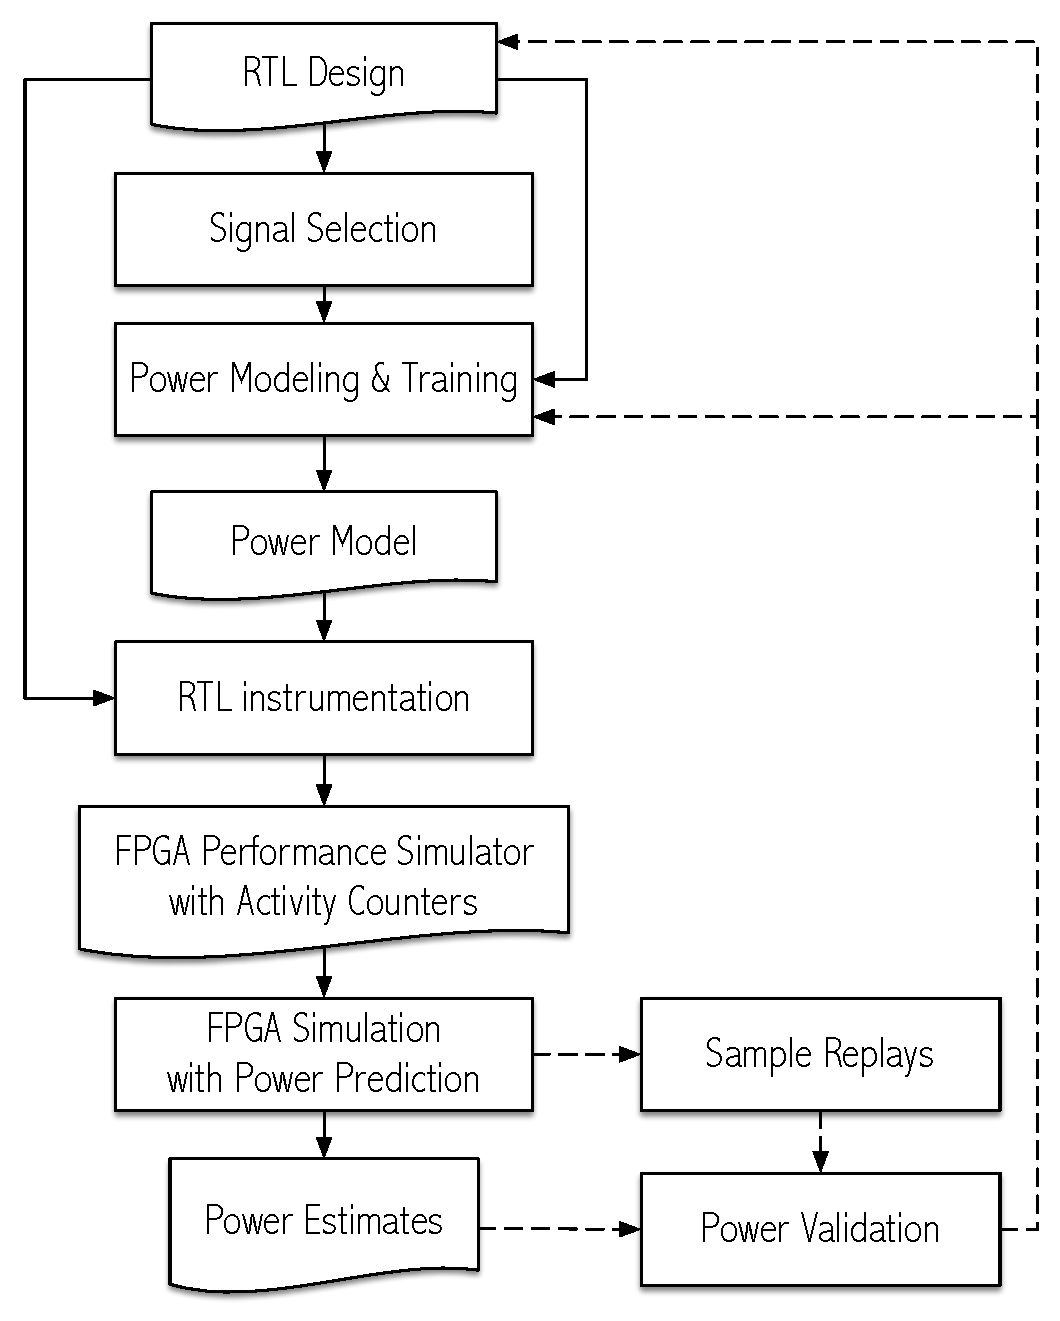
\includegraphics[width=0.4\textwidth,height=\textheight,keepaspectratio]{images/tool_flow.pdf}
	\caption{Overall Tool Flow}
	\label{fig:tool_flow}
\end{figure}

\subsection{Signal Selection}
\label{sec:signal_selection}

To construct and train a power model, we should select a subset of signals
because it is infeasible to keep track of all signal activities on the FPGA.

There are several observations to select power-sensitive signals. First of all,
\emph{the signal activities of the whole design are driven by the inputs and 
the state of the design.} Thus, we may be able to build an accurate power
model in terms of the register and input toggles. However, there are
a large number of registers in complex hardware designs, and thus,
this is still infeasible for the FPGA.

Fortunately, it seems that \emph{there are only a small number of signal activities
or/and high-level events that drive the state transitions of the design}.
Otherwise, all power estimation methods based on event counters~\cite{Bellosa2000,
Bircher2003, Isci2003,Bircher2005, Bircher2007, Bertran2013} do not make sense.
Therefore, we may be able to construct an accurate power model by using only
a small number of signals that approximate high-level performance / power events.

Figure~\ref{fig:signal_selection} describes how power sensitive signals
are selected. First of all, a random RTL design is fed into the FIRRTL compiler.
In this paper, we assume this design is written with Chisel~\cite{Bachrach2012}.
However, the target designs are not necessarily developed with Chisel
because the FIRRTL compiler will support various languages including Verilog in the near future.

In the FIRRTL compiler, a circuit graph is expressed with an intermediate representation,
FIRRTL~\cite{Li:EECS-2016-9}, so that a designer can write custom compiler passes for their
design. A signal analysis pass is implemented, which examines all write enable signals
for registers. For SRAMs, their write enable signals and read data busses are selected.
The selected signals and busses are dumped to the file used for
power model training in Section~\ref{sec:power_modeling}.

\begin{figure}[!ht]
	\centering
	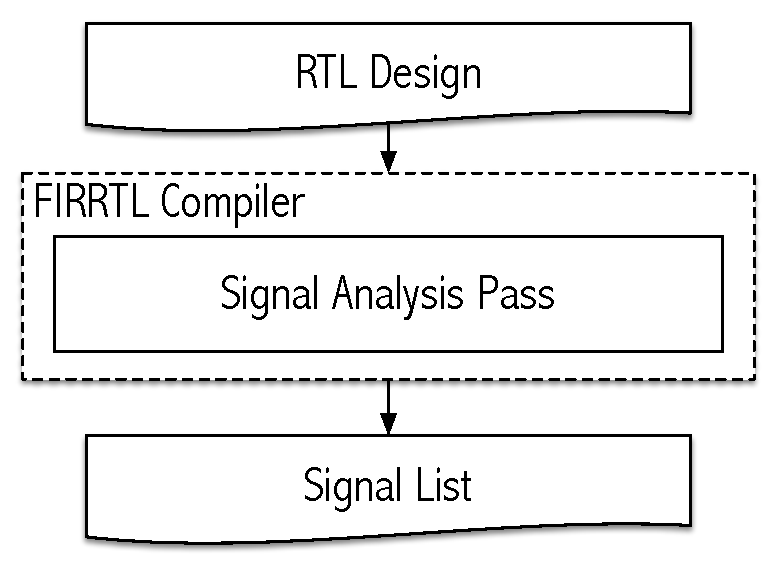
\includegraphics[width=0.35\textwidth,height=\textheight,keepaspectratio]{images/signal_selection.pdf}
	\caption{Signal Selection}
	\label{fig:signal_selection}
\end{figure}

\subsection{Power Modeling and Training}
\label{sec:power_modeling}
Once the signals and busses are selected from the previous step, 
a design-specific activity-based power model can be constructed.
Figure~\ref{fig:power_modeling} explains how power models are built and trained.
First, an RTL design is fed into the logic synthesis tool
(e.g. Synopsys Design Compiler~\textregistered) and the place-and-route tool
(e.g. Synopsys IC Compiler~\textregistered) to obtain a gate-level design,
which is simulated in SDF back-annotated gate-level simulation
(e.g. Synopsys VCS~\textregistered) for accurate power estimates
by the power analysis tool(e.g. Synopsys PrimeTime PX~\textregistered).

RTL signal activities are also computed from RTL simulation(e.g. Verilator, Synopsys VCS~\textregistered).
By providing the signal list, the RTL signal activities, and the detailed power estimates
to the power modeling and training algorithm, a design-specific power model can be constructed
expressed with the signal toggle activities.

For RTL simulation and gate-level simulation, microbenchmarks or random instruction streams are employed
for initial power model training. In addition, there can be random execution sample snapshots from
long-running FPGA performance simulation~\cite{Kim2016}, which are used not only for power model validation
but also for further training the power model for more accurate power estimates.

\begin{figure}[!ht]
	\centering
	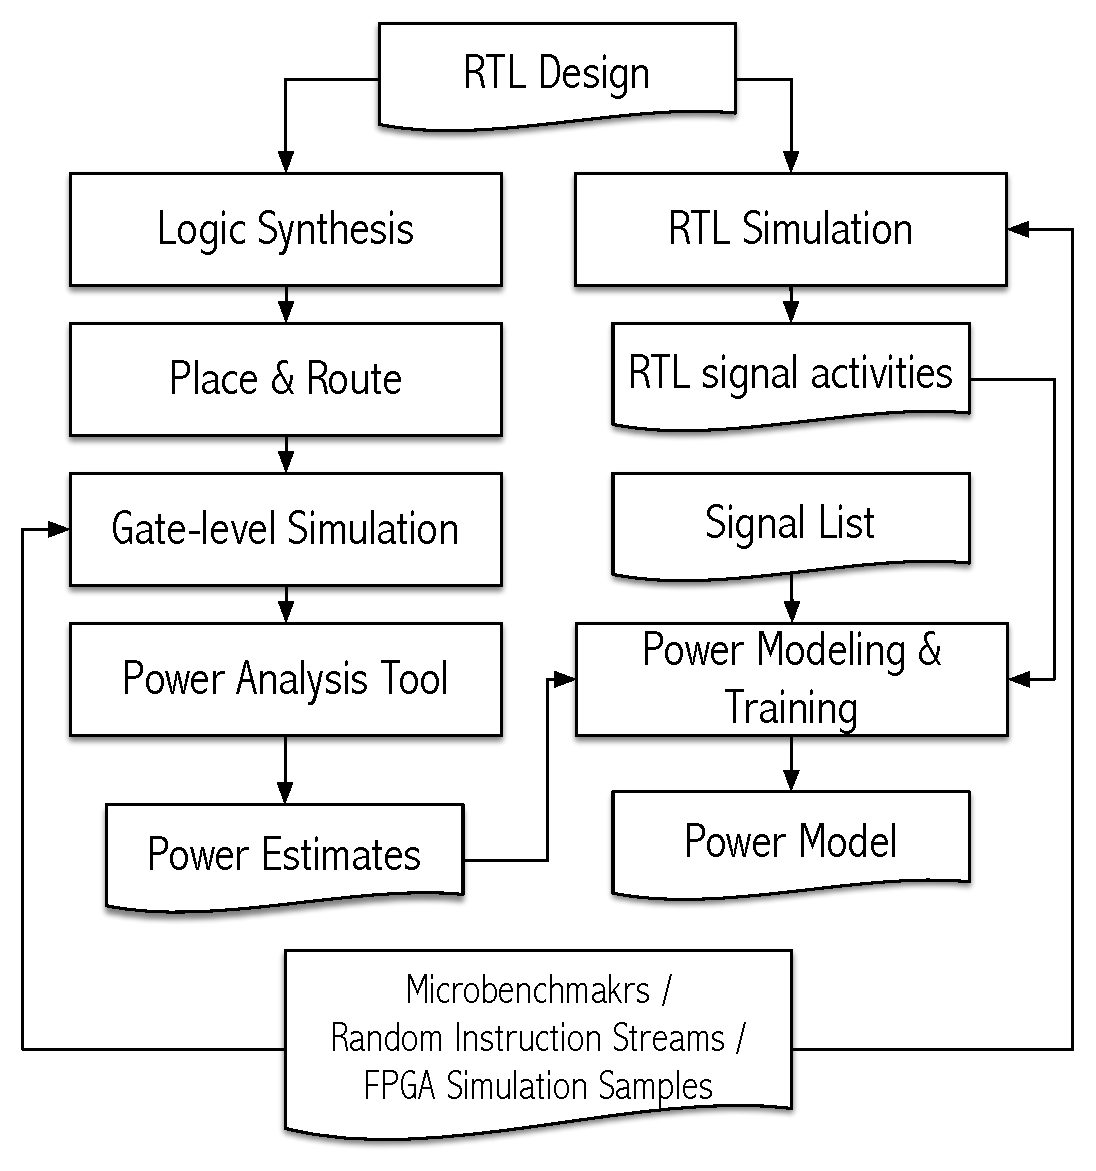
\includegraphics[width=0.4\textwidth,height=\textheight,keepaspectratio]{images/power_modeling.pdf}
	\caption{Power Modeling and Training}
	\label{fig:power_modeling}
\end{figure}

\subsubsection{Macromodels for Complex Combinational Logic}
Previous work~\cite{Sunwoo2010} suggests that linear power models for complex combinational logic such as ALUs, SEC/DED circuits, interrupt controllers, and multipliers are inaccurate. To overcome this issue, we turn to macromodels which attempt to estimate the power of complex logic by only looking at the input and output switching activity of the combinational block. In this paper we will measure the accuracy of a previously proposed power macromodel that uses 4 statistics $P_{in}, D_{in}, SC_{in}, D_{out}$.~\cite{Najm2000}\cite{Najm2000_2}

This macromodel considers sequences of input vectors into a combinational block. Each sequence may contain $N$ input vectors. Then we can define for a given sequence,
\begin{itemize}
	\item $P_{in}$ = average number of input bits that are logic 1 across a sequence
	\item $D_{in}$ = average number of input bit transitions across a sequence (average input transition density)
	\item $SC_{in}$ = average spacial correlation coefficient across a sequence and across all input bit pairs
	\item $D_{out}$ = average number of output bit transitions across a sequence (average output transition density)
\end{itemize}

In the context of power estimation for a large digital design: if a complex combinational block is detected in the design, the power macromodel will be used in place of a linear model. To feed the macromodel with data, the combinational block's inputs and outputs will be instrumented. A small logic block on the FPGA will map the raw input and output signals into a 4-tuple that represents the above statistics, and the tuple will be fed out of the FPGA emulator to be plugged into the power macromodel.

\subsection{RTL Instrumentation}
\label{sec:instrumentation}
The RTL instrumentation is built upon the Chisel3 and FIRRTL port of the Strober's flow
to generate FPGA performance simulators. Figure~\ref{fig:power_modeling} shows how
the FPGA performance simulators are instrumented with the signal activity counters.

First, the target RTL design is FAME1-transformed to create the FPGA performance simulator~\cite{Kim2016}
in the FIRRTL compiler. Then, a custom transform is executed to attach activity counters
to the FPGA performance simulator by using the signal list from Section~\ref{sec:signal_selection}.
In addition, scan chains are inserted not only to read out the activity counter values but also to
capture RTL state snapshots to validate the power model. Finally, simulation mapping and platform mapping
are conducted for FPGA simulation~\cite{Kim2016}.

Note that signal selection in Section~\ref{sec:signal_selection} can be integrated to
this flow if signals are not pruned during power modeling and training in
Section~\ref{sec:power_modeling}. In this case, FPGA simulation can run in parallel while
training power models, which uses slow CAD tools extensively.

\begin{figure}[!ht]
	\centering
	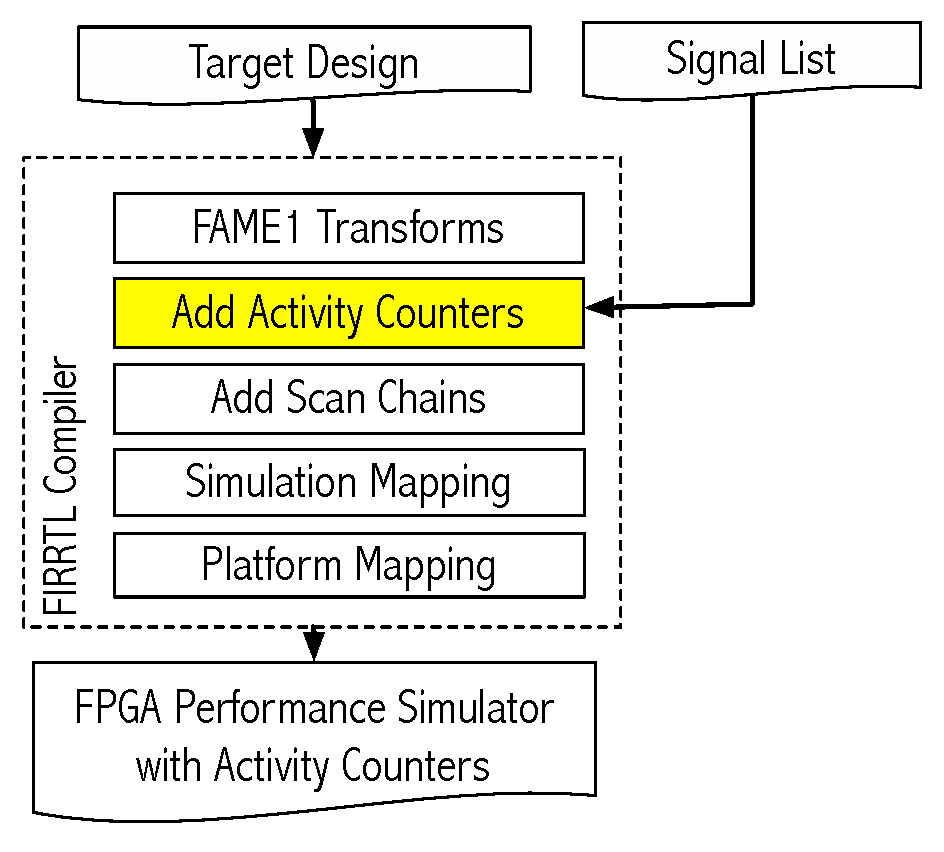
\includegraphics[width=0.4\textwidth,height=\textheight,keepaspectratio]{images/instrumentation.pdf}
	\caption{Power Modeling and Training}
	\label{fig:power_modeling}
\end{figure}

\subsection{Power Prediction during FPGA Simulation}
\label{sec:power_prediction}
Once the FPGA performance simulator instrumented with activity counters is obtained,
power estimates are quickly available during FPGA simulation. Since the target RTL
is FAME1-transformed, FPGA simulation can be easily paused, and activity counter
values are read out from the FPGA in the same way random RTL state sample snapnots
are taken in Strober~\cite{Kim2016}. If the power model is not available during
FPGA simulation because it is still trained, the activity counter values are saved
to estimate the power dissipation later.

\subsection{Power Validation}
\label{sec:power_validation}
Designers may want to validate the power estimates from Section~\ref{sec:power_prediction}
after FPGA simulation. Since this methodology is combined with Strober,
an accurate power estimates with statistically bounded errors are available by
replaying random RTL state snapshots, which are used to further train the power model
for more accurate power estimates (Figure~\ref{fig:power_modeling}).


\section{Experimental Setup and Results}
\subsection{Power Macromodel for Combinational Logic}
To validate the accuracy of the power macromodel proposed in~\cite{Najm2000_2}, we will generate multiple sequences of input training vectors, derive an accurate power estimate from PrimeTime, and use the statistics ($P_{in}, D_{in}, SC_{in}, D_{out}$) associated with each sequence to train the macromodel. We will then generate a separate set of sequences which will be used to test the macromodel's accuracy as compared to the PrimeTime power estimate.

The combinational circuits used in this study were the following ISCAS 85 benchmark circuits:

\begin{itemize}
	\item \textit{c17}: 6 NAND gates
	\item \textit{c432}: 27-channel interrupt controller
	\item \textit{c499}: 32-bit SEC
	\item \textit{c880}: 8-bit ALU
	\item \textit{c1908}: 16-bit SEC/DED
	\item \textit{c2670}: 12-bit ALU
	\item \textit{c6288}: 16x16 multiplier
	\item \textit{c7552}: 32-bit adder/comparator 
\end{itemize}

The training and testing datasets consisted of 300 sequences of 30 vectors. They were run through the DUT using RTL simulation and post-PAR gate-level simulation. The gate-level simulations were used to derive switching activity files which when passed to PrimeTime PX gave a power estimate for a given sequence. Using the input and output vectors, and the power estimate from PrimeTime the 4 following power macromodels were constructed:

\begin{itemize}
	\item \textit{4D Table}: A simple map from a $P_{in}, D_{in}, SC_{in}, D_{out}$ vector to a power estimate.
	\item \textit{Linear Model}: Coefficients were derived for an equation of the form $c_0 + c_1 P_{in} + c_2 D_{in} + c_3 SC_{in} + c_4 D_{out}$ using least squares regression. (5 coefficients)
	\item \textit{Quadratic Model}: Coefficients were derived for an equation consisting of the linear terms, but also cross terms and self-squared terms using least squares regression. (15 coefficients)
	\item \textit{Cubic Model}: Added triplet cross terms and self-cubed terms. (35 coefficients)
\end{itemize}

Once the models were constructed and trained using the training dataset, they were used to make predictions on the testing dataset.

4D table prediction involves interpolating new ($P_{in}, D_{in}, SC_{in}, D_{out}$) vectors on the training dataset: if interpolation wasn't possible due to the testing vector being outside the convex hull of the training vectors, then the nearest neighbor's power estimate was used. Prediction on the linear, quadratic, and cubic models was performed with simple matrix multiplication of the testing vectors and the previously calculated coefficients.

Errors in the the macromodel were measured and are summarized in Figure \ref{fig:rms_error} and Figure \ref{fig:max_error}.

\begin{figure*}
	\centering
	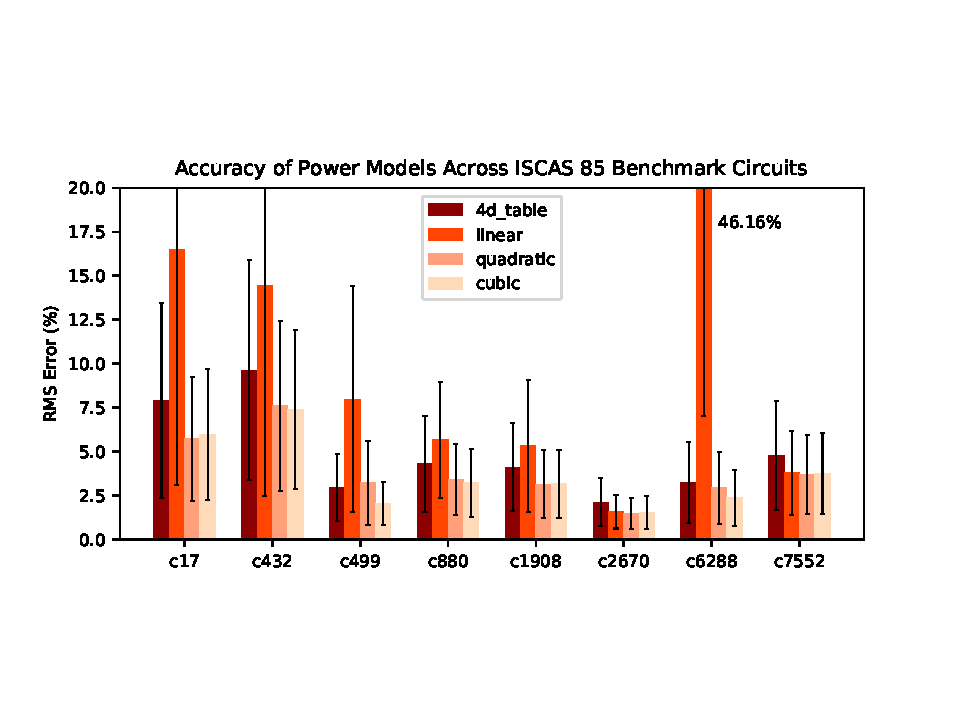
\includegraphics[clip, trim=0.5cm 2.5cm 0.5cm 2.5cm,width=0.85\textwidth,height=\textheight,keepaspectratio]{images/error_plot.pdf}
	\caption{RMS errors from macromodel power estimation, error bars indicate 1 SD}
	\label{fig:rms_error}
\end{figure*}

\begin{figure*}
	\centering
	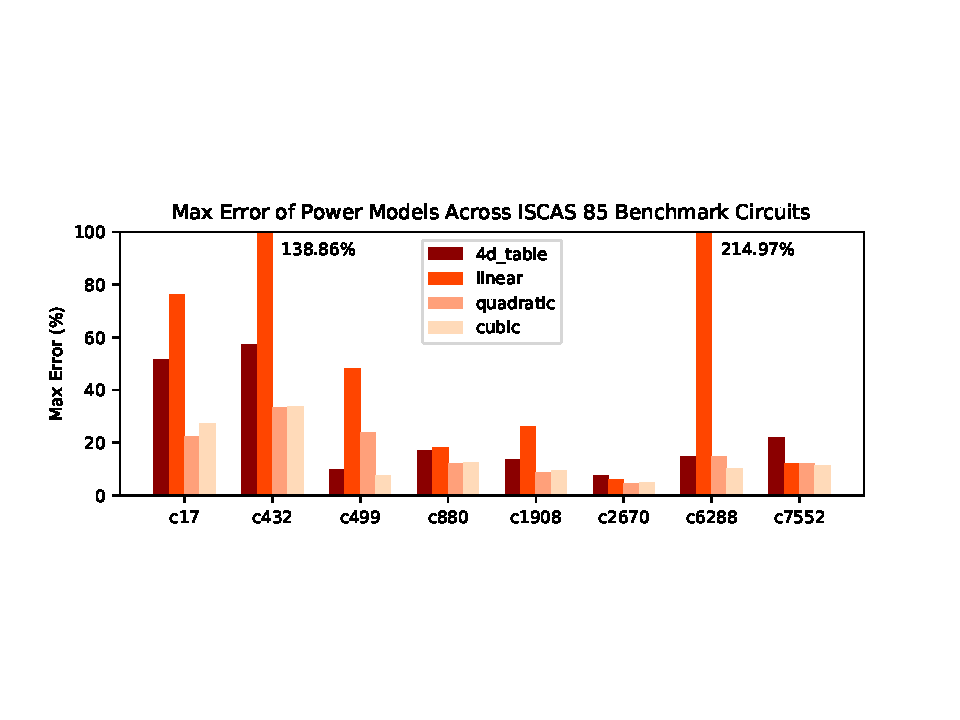
\includegraphics[clip, trim=0.5cm 3cm 0.5cm 3cm,width=0.85\textwidth,height=\textheight,keepaspectratio]{images/max_error_plot.pdf}
	\caption{Max errors from macromodel power estimation, worst case accuracy}
	\label{fig:max_error}
\end{figure*}

\subsection{Sequential Circuit Power Modeling}

To demonstrate the capability of the automatic signal section methodology for sequential logic,
we evaluate our methodology using simple Chisel designs described as follows:

\begin{itemize}
	\item \textit{GCD}: hardware implementation of Euclidean algorithm
	\item \textit{Parity}: computation for the parity of inputs
	\item \textit{Stack}: hardware implementation of stack
	\item \textit{Risc}: very simple single-cycle pipeline
	\item \textit{RiscSRAM}: very simple multi-cycle pipeline with SRAMs
\end{itemize}

We run 20 sets of simulation to train the power models and use different 20 sets of simulation
to test the power models. Quadratic models are used for \emph{GCD} and \emph{Parity}, and 
cubic models are used for \emph{Stack}, \emph{Risc}, and \emph{RiscSRAM}. 
Table~\ref{tbl:results} shows the power model errors for the designs. The maximum error of
\emph{Stack} is somewhat warrisome, but we may address it by having more training sets.
Impressively, this methodology works well for more complex designs like \emph{Risc} and \emph{RiscSRAM}.

\begin{table*}
\begin{center}
  \begin{tabular}{ | c | c | c | c | c | c |}
    \hline
    \textbf{Design} & \textbf{GCD} & \textbf{Parity} & \textbf{Stack} & \textbf{Risc} & \textbf{RiscSRAM} \\ \hline
	\textbf{Number of Selected Signals and Busses} & 7 & 3 & 8 & 11 & 15 \\ \hline
	\textbf{Normalized RMS error(\%)} &  29.3 & 1.9 & 31.9 & 4.0 & 10.0 \\ \hline
	\textbf{Average error(\%)}        &   5.1 & 0.9 & 26.9 & 2.3 & 6.5 \\ \hline
	\textbf{Maximum error(\%)}        &  16.5 & 2.4 & 153.7 & 7.4 & 20.5 \\ \hline

  \end{tabular}
  \caption{Evaluation with Examples}
  \label{tbl:results}
\end{center}
\end{table*}

To demonstrate how well signal selection works, we use a more complex design, RISCV-mini~\cite{riscv-mini}. 
RISCV-mini implements RV32I of the User-level ISA Version 2.0~\cite{riscv-user-2.0} and
the Machine-level ISA of the Privileged Architecture Version 1.7~\cite{riscv-prev-1.7}.
RISCV-mini includes a 3-stage pipeline as well as instruction and data caches as shown
in Figure~\ref{fig:riscv_mini}, which is neither too simple nor too complex.
From RISCV-mini, 108 signals are selected. However, about 50~\% of theses signals
are due to lack of inter-module analysis, which will be cut out from pass optimization.

\begin{figure}
 	\centering
 	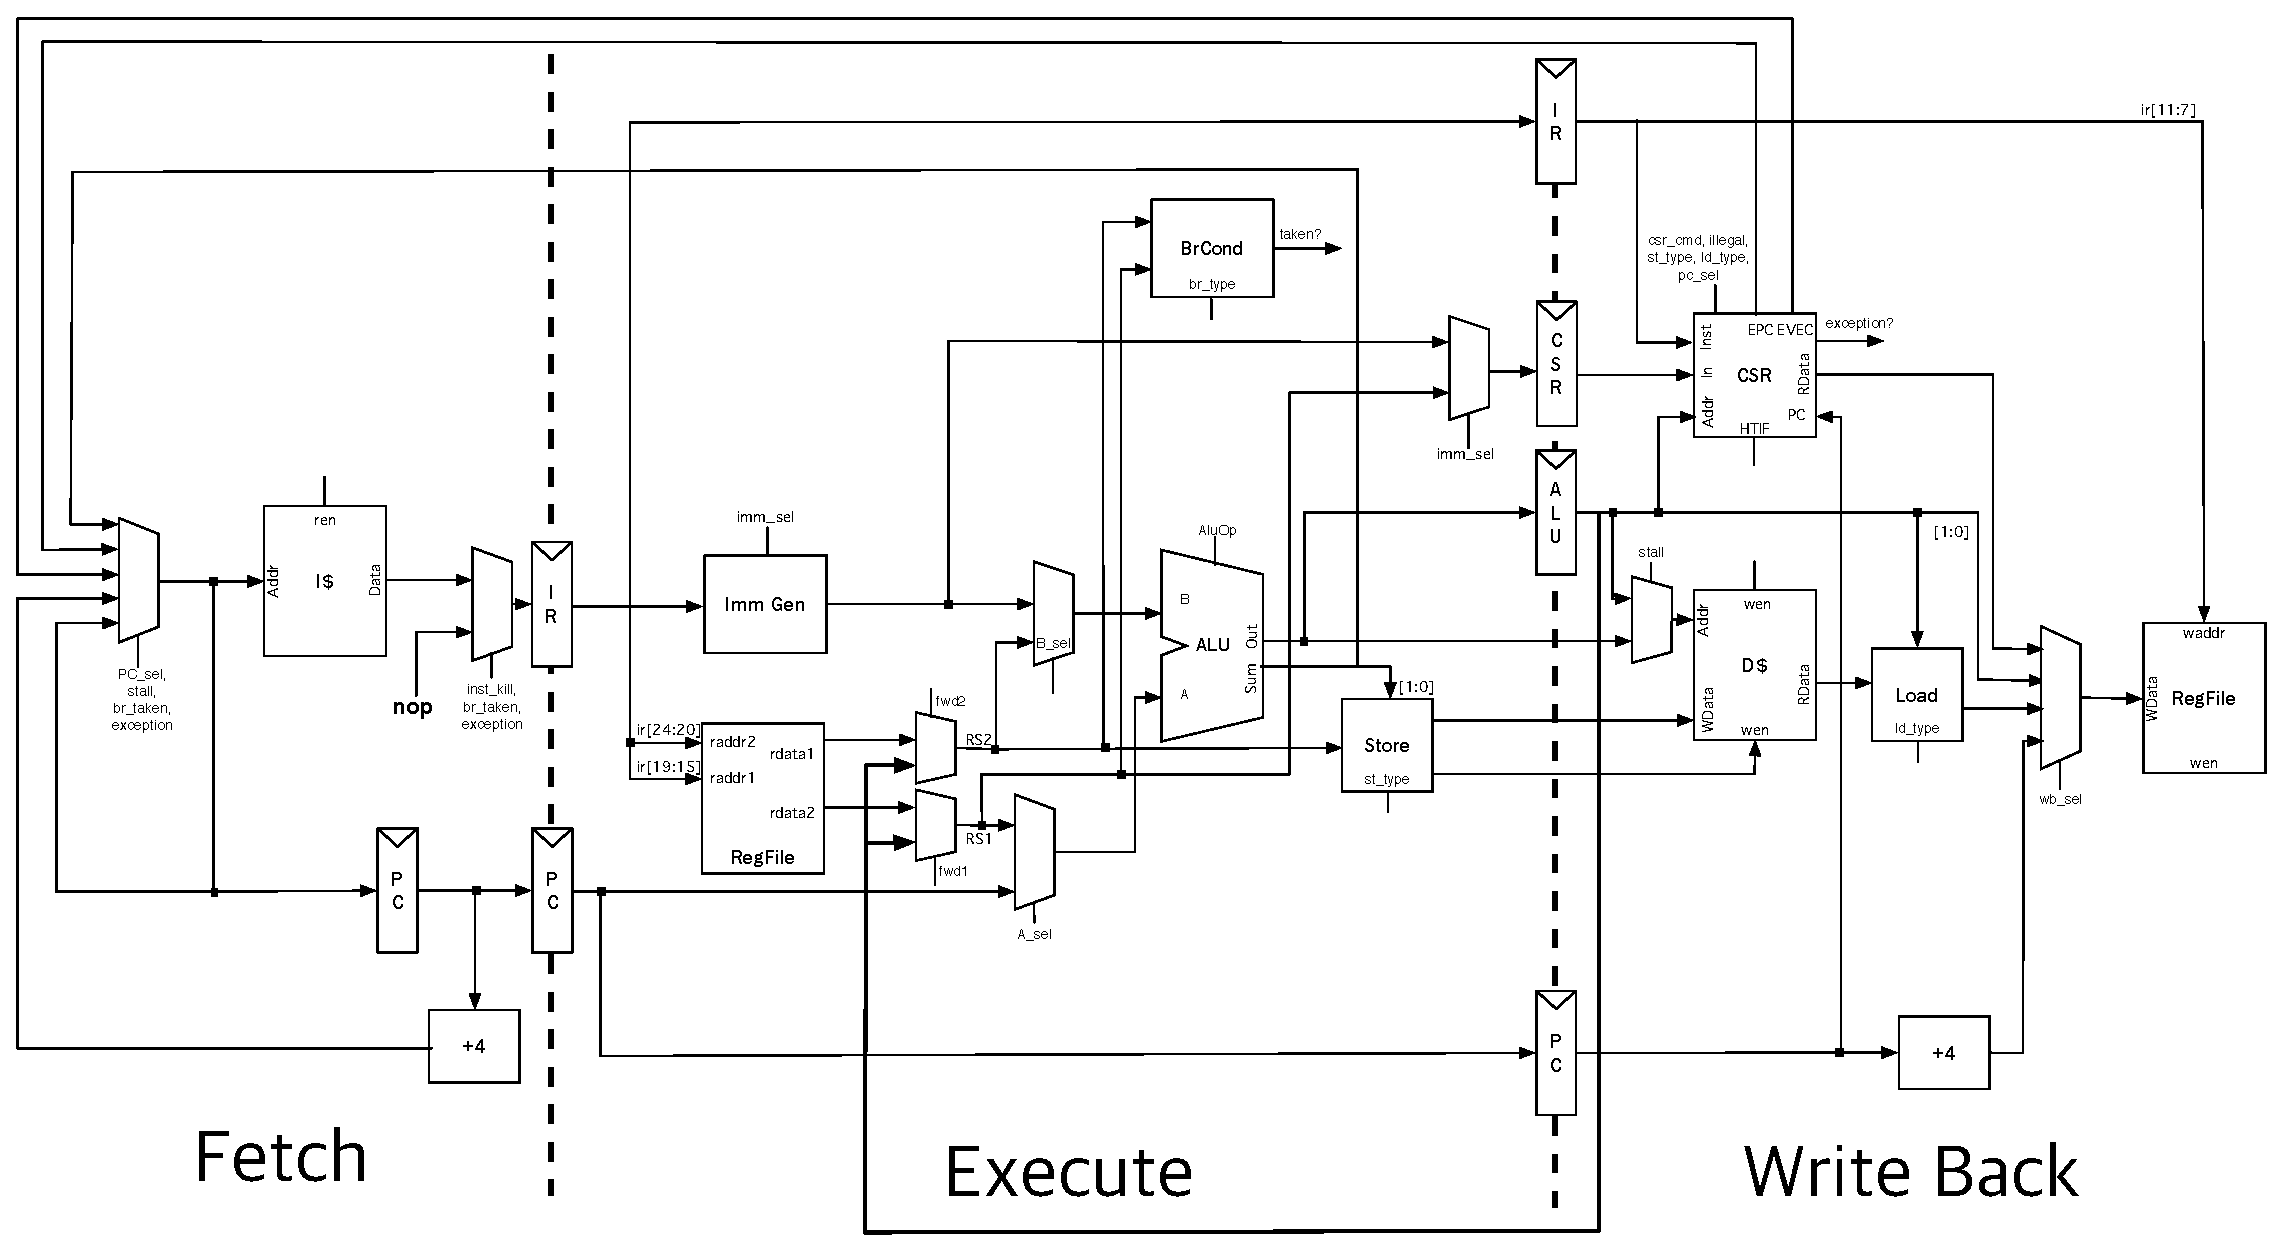
\includegraphics[width=\columnwidth,height=\textheight,keepaspectratio]{images/riscv_mini.pdf}
 	\caption{RISCV-mini Pipeline}
 	\label{fig:riscv_mini}
\end{figure}

% An example of a floating figure using the graphicx package.
% Note that \label must occur AFTER (or within) \caption.
% For figures, \caption should occur after the \includegraphics.
% Note that IEEEtran v1.7 and later has special internal code that
% is designed to preserve the operation of \label within \caption
% even when the captionsoff option is in effect. However, because
% of issues like this, it may be the safest practice to put all your
% \label just after \caption rather than within \caption{}.
%
% Reminder: the "draftcls" or "draftclsnofoot", not "draft", class
% option should be used if it is desired that the figures are to be
% displayed while in draft mode.
%
%\begin{figure}[!t]
%\centering
%\includegraphics[width=2.5in]{myfigure}
% where an .eps filename suffix will be assumed under latex, 
% and a .pdf suffix will be assumed for pdflatex; or what has been declared
% via \DeclareGraphicsExtensions.
%\caption{Simulation results for the network.}
%\label{fig_sim}
%\end{figure}

% Note that the IEEE typically puts floats only at the top, even when this
% results in a large percentage of a column being occupied by floats.


% An example of a double column floating figure using two subfigures.
% (The subfig.sty package must be loaded for this to work.)
% The subfigure \label commands are set within each subfloat command,
% and the \label for the overall figure must come after \caption.
% \hfil is used as a separator to get equal spacing.
% Watch out that the combined width of all the subfigures on a 
% line do not exceed the text width or a line break will occur.
%
%\begin{figure*}[!t]
%\centering
%\subfloat[Case I]{\includegraphics[width=2.5in]{box}%
%\label{fig_first_case}}
%\hfil
%\subfloat[Case II]{\includegraphics[width=2.5in]{box}%
%\label{fig_second_case}}
%\caption{Simulation results for the network.}
%\label{fig_sim}
%\end{figure*}
%
% Note that often IEEE papers with subfigures do not employ subfigure
% captions (using the optional argument to \subfloat[]), but instead will
% reference/describe all of them (a), (b), etc., within the main caption.
% Be aware that for subfig.sty to generate the (a), (b), etc., subfigure
% labels, the optional argument to \subfloat must be present. If a
% subcaption is not desired, just leave its contents blank,
% e.g., \subfloat[].


% An example of a floating table. Note that, for IEEE style tables, the
% \caption command should come BEFORE the table and, given that table
% captions serve much like titles, are usually capitalized except for words
% such as a, an, and, as, at, but, by, for, in, nor, of, on, or, the, to
% and up, which are usually not capitalized unless they are the first or
% last word of the caption. Table text will default to \footnotesize as
% the IEEE normally uses this smaller font for tables.
% The \label must come after \caption as always.
%
%\begin{table}[!t]
%% increase table row spacing, adjust to taste
%\renewcommand{\arraystretch}{1.3}
% if using array.sty, it might be a good idea to tweak the value of
% \extrarowheight as needed to properly center the text within the cells
%\caption{An Example of a Table}
%\label{table_example}
%\centering
%% Some packages, such as MDW tools, offer better commands for making tables
%% than the plain LaTeX2e tabular which is used here.
%\begin{tabular}{|c||c|}
%\hline
%One & Two\\
%\hline
%Three & Four\\
%\hline
%\end{tabular}
%\end{table}


% Note that the IEEE does not put floats in the very first column
% - or typically anywhere on the first page for that matter. Also,
% in-text middle ("here") positioning is typically not used, but it
% is allowed and encouraged for Computer Society conferences (but
% not Computer Society journals). Most IEEE journals/conferences use
% top floats exclusively. 
% Note that, LaTeX2e, unlike IEEE journals/conferences, places
% footnotes above bottom floats. This can be corrected via the
% \fnbelowfloat command of the stfloats package.


\section{Conclusion}
In this report, a novel approach to accurately and quickly predict
cycle-level power estimates for arbitrary RTL was presented.
Import signals sensitive to power dissipation were automatically
selected using a custom analysis pass in the FIRRTL compiler.
Also, power models were built and trained using the signal list,
the RTL signal activities, and the accurate power estimates
from detailed gate-level simulation. The RTL instrumentation
was done on top of the Strober's flow for the FPGA performance
simulators to automatically add activity counters using the
signal list. During FPGA simulation, online power prediction
was readily obtained by pausing the simulation and reading out
the activity counters. Finally, the power model was validated
and further trained by replaying random RTL state snapshots.

One possible application of this methodology is fast DVFS
modeling using FPGA simulation. To enable DVFS in simulation,
online power prediction must be available for the
power management unit model to control voltage and
frequency. By using this methodology, it is expected
we will simulate DVFS with FPGA performance simulatros
in the near future.

% conference papers do not normally have an appendix


% use section* for acknowledgment
%\section*{Acknowledgment}


% trigger a \newpage just before the given reference
% number - used to balance the columns on the last page
% adjust value as needed - may need to be readjusted if
% the document is modified later
%\IEEEtriggeratref{8}
% The "triggered" command can be changed if desired:
%\IEEEtriggercmd{\enlargethispage{-5in}}

% references section

% can use a bibliography generated by BibTeX as a .bbl file
% BibTeX documentation can be easily obtained at:
% http://mirror.ctan.org/biblio/bibtex/contrib/doc/
% The IEEEtran BibTeX style support page is at:
% http://www.michaelshell.org/tex/ieeetran/bibtex/
%\bibliographystyle{IEEEtran}
% argument is your BibTeX string definitions and bibliography database(s)
%\bibliography{IEEEabrv,../bib/paper}
%
% <OR> manually copy in the resultant .bbl file
% set second argument of \begin to the number of references
% (used to reserve space for the reference number labels box)
\bibliographystyle{ieeetr}
\bibliography{ref}

% that's all folks
\end{document}


